\section{Domain model}
\begin{comment}
Give a high level view overview of the application using a UML diagram.
\end{comment}
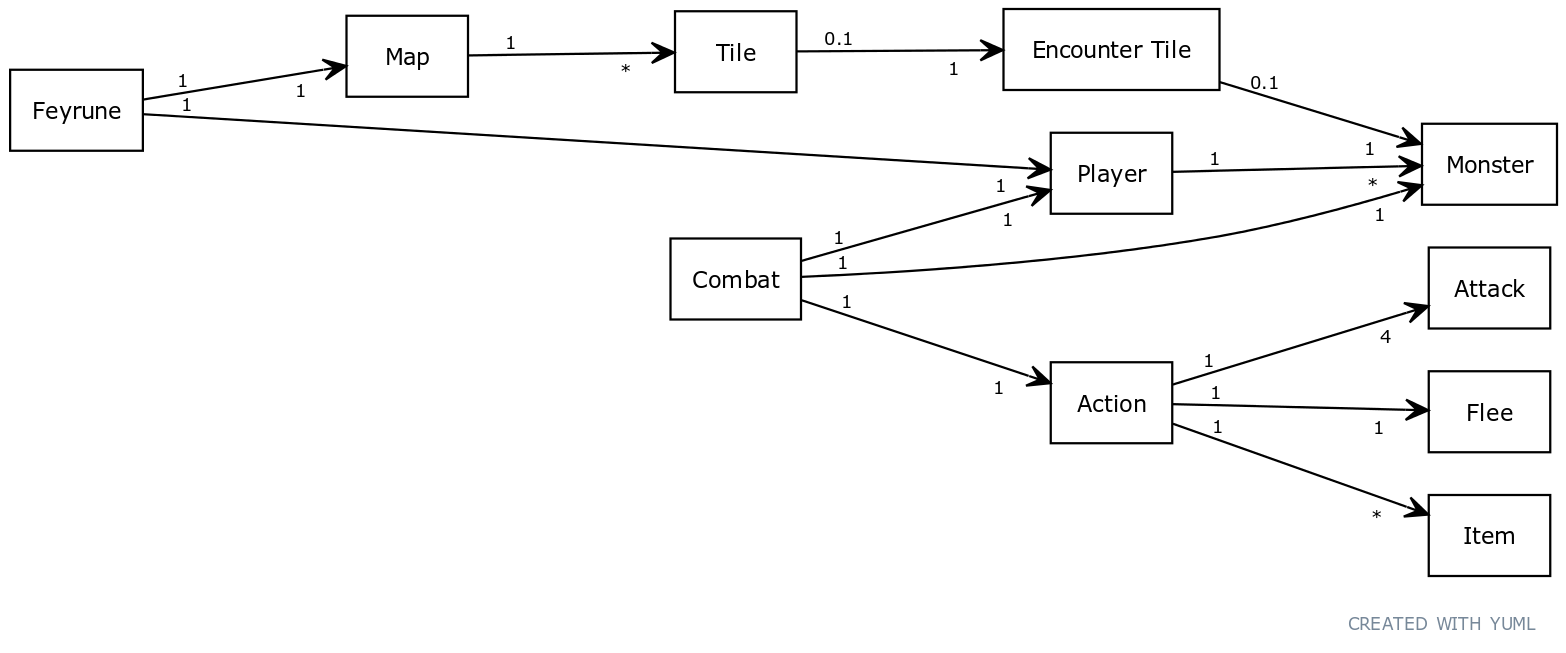
\includegraphics[width=\textwidth]{images/domain_model.png}

\subsection{Class responsibilities}
\begin{comment}
Explanation of responsibilities of classes in diagram.
\end{comment}
    \paragraph{Feyrune}
    ~\\\indent\indent Feyrune is the name of our game/ application and is the main program.
    \paragraph{Map}
    ~\\\indent\indent Map is a tiled map that has information about all that the can be seen and explored in the world
    \paragraph{Tile}
    ~\\\indent\indent A tile is a small part of the map that has information about what that specific tile, ex graphics, collision and encounter
    \paragraph{Encounter Tile}
    ~\\\indent\indent The Encounter Tile can with chance start a combat with generates a monster and takes information about the players owned monsters
    \paragraph{Player}
    ~\\\indent\indent The Player has a collection of monsters, some paragraph{}s and a position on the Map. The player is also what you as a user can control.
    \paragraph{Combat}
    ~\\\indent\indent The combat has one enemy and a players monster that fight until death or someone flees. There are a number of actions that both the enemy monster and the players monster can do
    \paragraph{Action}
    ~\\\indent\indent An action is what you or the enemy can do in a combat
    \paragraph{Monster}
    ~\\\indent\indent A monster is a creature with stats and is the cornerstone of this application
    \paragraph{Attack}
    ~\\\indent\indent All monsters can have one to four different attacks that have different effects on the combat or simply do different amounts of damage.
    \paragraph{Flee}
    ~\\\indent\indent The flee action lets you have a chance to leave the combat without having to fight until death.
    \paragraph{Item} %TODO: Have we even added items to the game yet?
    ~\\\indent\indent An item is a separate action from an attack that can have different effect on the combat.